% !TEX root = ../thesis.tex
%
\chapter{Our method}
\label{sec:pipeline}
In this chapter we explain how we build our network from \gls{resnet} and under which conditions we train it \tref{sec:pipeline:training}. Next we show how we generate bounding box object predictions on top of the pixel-wise class probabilities \tref{sec:pipeline:eval}.

\section{Training}
\label{sec:pipeline:training}
We use the \gls{resnet}-50 \tref{sec:concepts:resnet:design} as the basis for our detector and take the pretrained model\footnote{\url{https://github.com/KaimingHe/deep-residual-networks\#models}} that is provided by the original authors. They trained the network on the 1000 classes of the ImageNet 2012 dataset \citep{russakovsky_imagenet_2015} and therefore we can assume that the learned features are good class-independent image descriptors. For our single-class detection we replace the original \gls{fc} layer with a new one, now only returning two values (background \textit{vs} foreground).\\
As we aim for fast \textit{approximate} training on a single class, it is not feasible to retrain or refine any of the \gls{conv} layers and instead we only train the weights of the single \gls{fc} layer. Additionally refining the last \gls{conv} layers in the same restricted number of iterations did not yield considerable better results.\\
We want to use an \gls{fcn} to provide localized object predictions. This is done by the classifier to \gls{fcn} conversion described in \treft{sec:concepts:fcn}. The classifying \gls{resnet} is transformed by converting the \gls{fc} layer into a \gls{conv} layer after training and appending an upsampling operation of the sparse prediction map. Following the results of \citep{shelhamer_fully_2016}, we do not train the upsampling and use fixed bilinear weights. Again the new \gls{conv} layer could be refined on the pixel level using segmentation maps but under our self-imposed restrictions the further training did not result in considerable success.

For optimizing we use \gls{sgd} with momentum of 0.9. The weight decay is set at 0.0001 and the learning rate fixed at \num{1e-6}. Employing a learning rate reduction method, like reducing after fixed steps, did not influence training results and is thus omitted. Because we want time limited training we abort training independent from any validation measure after 500 iterations. Thereby we guarantee constant time complexity in training. The fixed number of iterations was chosen after multiple test with shorter and longer training durations.

\subsection{Preprocessing and augmentation}
\label{sec:pipeline:training:augment}
\begin{figure}[htb]
    \begin{tabularx}{\textwidth}{XXXXX}
        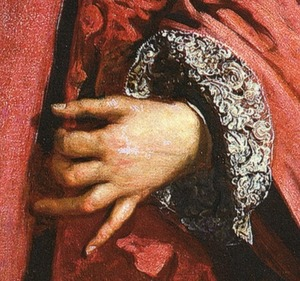
\includegraphics[width=0.170\textwidth]{figures/aug/parts_example} &
        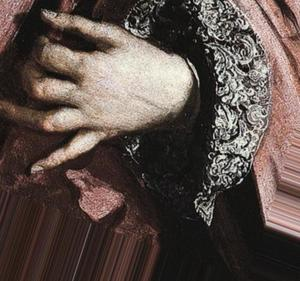
\includegraphics[width=0.170\textwidth]{figures/aug/parts_example_2} &
        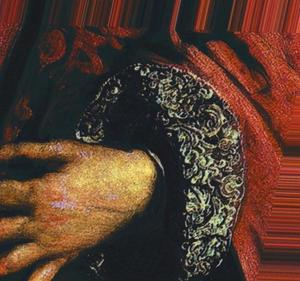
\includegraphics[width=0.170\textwidth]{figures/aug/parts_example_18} &
        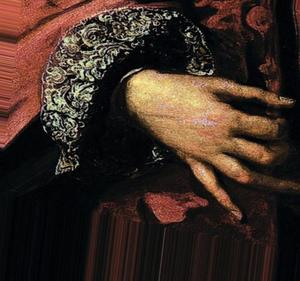
\includegraphics[width=0.170\textwidth]{figures/aug/parts_example_19} &
        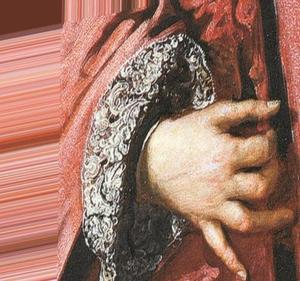
\includegraphics[width=0.170\textwidth]{figures/aug/parts_example_5} \\

        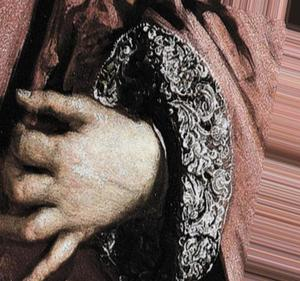
\includegraphics[width=0.170\textwidth]{figures/aug/parts_example_6} &
        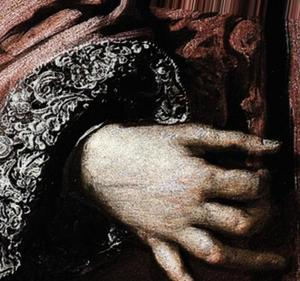
\includegraphics[width=0.170\textwidth]{figures/aug/parts_example_7} &
        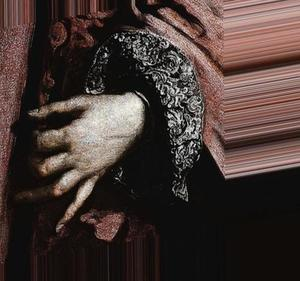
\includegraphics[width=0.170\textwidth]{figures/aug/parts_example_8} &
        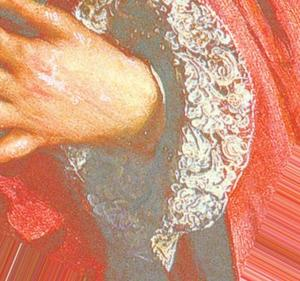
\includegraphics[width=0.170\textwidth]{figures/aug/parts_example_9} &
        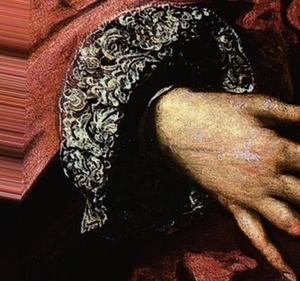
\includegraphics[width=0.170\textwidth]{figures/aug/parts_example_10}
    \end{tabularx}
	\caption{Top-left is the original patch and the other ones are transformed samples. Painting sample is from the \textit{Portrait of the Procurator Giolamo Querini} by Bombelli, Sebastino \citep{bombelli_retrato_1669}.}
    \label{fig:augmentation}
\end{figure}
It has long been shown that preprocessing the training data and expanding it by modifying the data improves training time and test results \citep{dosovitskiy_discriminative_2014}.\\
We preprocess the training samples $I_k$ with only one step, by subtracting the mean of all images of the dataset from each sample \citep{krizhevsky_imagenet_2012}. Through this step the input data becomes zero-centered.\\
Moreover as we will increasingly reduce the number $k$ of samples to train from, data augmentation is immensely important.  We employ multiple image transformations to artificially enlarge the training set. For this we use the preprocessing methods provided by the Keras library \citep{chollet_keras:_2015} and add additional transformations. Generating new samples is done with a set of bounded transformations. The composite transformation $T_p$ is chosen with the parameter vector $p = \{\alpha, \beta, s, t_x, t_y, m, t_s, t_v, f_s, f_v, v_s, v_v\}$ defining the following transformations which are applied in the given order:
\begin{my_list_item}
    \item \textbf{Rotation} with $\alpha\in[-\ang{20}, +\ang{20}]$
    \item \textbf{Translation} with $t_x,t_y\in[-\SI{5}{\percent}, \SI{5}{\percent}]$ of the patches' size in either directions on both axes.
    \item \textbf{Shearing} with $\beta\in[-\ang{11.5}, + \ang{11.5}]$
    \item \textbf{Zoom} with $s\in[\SI{70}{\percent}, \SI{130}{\percent}]$
    \item \textbf{Flipping} horizontally $m\in\{0,1\}$.
    \item \textbf{Contrast}. Patches are converted to the HSV color space. We raise saturation and value to a power $t_s, t_v \in [0.25, 4]$, then multiply by factors $f_s, f_v \in [0.7, 1.4]$, and add these to some values $v_s, v_v \in [-0.1, 0.1]$ \citep{dosovitskiy_discriminative_2014}. After the contrast transformation patches are again converted back to RGB color space.
\end{my_list_item}
Some examples of transformed images under those boundaries are seen in \figreft{fig:augmentation}. The parameter boundaries were chosen similar to those in \citet{dosovitskiy_discriminative_2014}. While training, the image generator picks random images from the training set, processes each image using a random parameter vector and returns the transformed images online. Finally they are resized to a size of $224\times 224$ pixels and fed into the network.

Because the generation of new augmented samples severely slows down training if done on demand we generate new samples in parallel to the network training on the CPU.

For good training performance we need a balanced set of positive samples and negative background samples. Therefore we want to feed the image augmenter a balanced set of seed patches. We enlarge the set of positive seed samples by initial randomly translated patches around each $i\in I_k$ with $t_{x'},t_{y'}\in[-\SI{25}{\percent}, \SI{25}{\percent}]$. This also has the advantage, that the image augmenter additionally receives the surroundings of the original query box. Depending on the set size $k$ we get $ppI$ number of seed samples from each image $i$ and take the same number of negative seed samples. Thereby we have at last $n = 2\cdot k \cdot ppI$ input samples for the generator.

\section{Generating detections}
\label{sec:pipeline:eval}
Our desired output of the algorithm is one or are multiple boxes $B=\{b_0,\dotsc,b_n\}$ enclosing each a section of the image $I$, which are predicted to contain the object that was searched for. The \gls{fcn} returns a score map $M$ as output. Each score $m_{i,j}\in M$ predicts the probability of this pixel $(i,j)$ to belong to the class $c$ we trained for. Therefore we need a method $g(M) = B$ to return high scoring bounding boxes from a probability map. The way of doing this used here consists of multiple steps:\\
\begin{my_list_num}
    \item We penalize (near-) empty regions inside the probability map with a negative distance transform
    \item We generate a set of boxes on a regular grid over the image shape
    \item For all those boxes we calculate their density of scores
    \item We apply a low threshold to filter out unnecessary boxes
    \item We apply \gls{nms} to get the top scoring boxes
\end{my_list_num}
In the following sections we explain each step in depth.

\subsection{Negative Distance Transform}
\label{sec:pipeline:eval:dt}
\begin{figure}[htb]
    \begin{tabular}{ccc}
        A probability map & Thresholded map & Distance transform \\[3pt]
        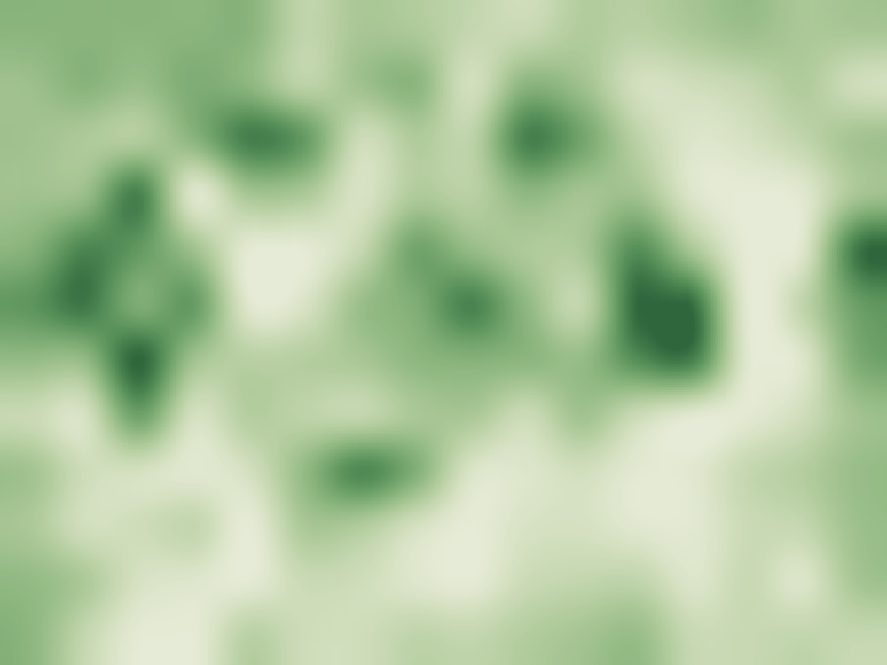
\includegraphics[width=0.303\textwidth]{figures/distance_transform_hm} &
        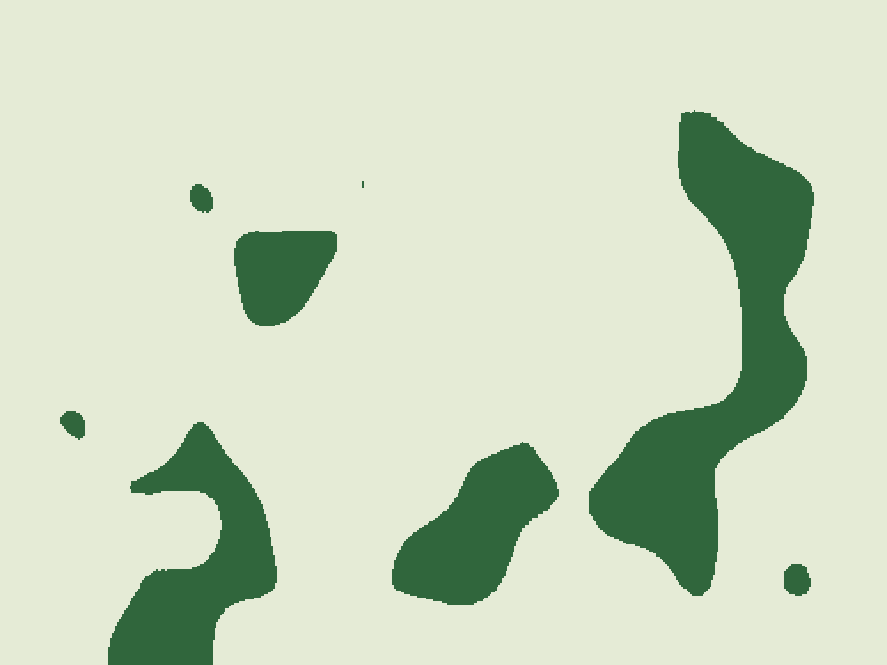
\includegraphics[width=0.303\textwidth]{figures/distance_transform_thres} &
        
\includegraphics[width=0.303\textwidth]{figures/distance_transform_negative}
    \end{tabular}
	\caption{Computing the negative distance transform from a probability map}
    \label{fig:distance_transform}
\end{figure}
Many images produce probability maps $M$, that are sparsely filled. Positive regions receive a positive score from the network, while non-positive regions are at-most zero. Thus the maps contain flat regions of constant value. We want to score the inner lying values of flat regions negatively, compared to boundary values. Here we introduce a distance transform to, sort of, impress those regions \fref{fig:distance_transform}.\\
First we threshold the score map with a near-zero value to set all values, that can safely assumed to be negatives, to zero.\\
Second we apply a distance transform to the mask $M'$ that resulted from the thresholding. A distance transform fills each zero pixel of the mask with its distance to the nearest one valued pixel. The distances are calculated with some metric, like the Euclidean distance or the $L_1$ distance. As the specific metric is not important for our vague penalizer and as we aim for good time performance we use the $L_\infty$ distance, also known as the chessboard distance. For our 2-dimensional image space the metric defines the distance between two points $(x_1, y_1)$ and $(x_2, y_2)$ as follows:
\begin{equation}
    L_\infty = \max(|x_2 - x_1|, |y_2 - y_1|)
\end{equation}
The transformed image is normalized and substracted from the original probability map. This additional step increases mean \gls{auc} on the \textsc{Pascal}-Part by 2\% for sets with $< 25$ images.\\
Nevertheless does this additional computation slow down the image processing and with only a marginal improvement this step probably can be omitted in live applications.

\clearpage
\subsection{Calculating the score densities}
\label{sec:pipeline:eval:density}
For each processed image we generate a set of boxes to calculate the score densities for. At three scales we take boxes $B = \{b_1,\dotsc, b_i = (x_0, y_0, x_1, y_1)_i,\dotsc, b_k\}$ with three different aspect ratios for $k=9$ \citep{ren_faster_2015} proposals at each position. We slide these anchor boxes  with overlapping stride over the image and collect the resulting slices. Also we save the areas $\{A_1,\dotsc, A_i,\dotsc\}$ for all rectangles.\\
Density is calculated by summing up all the probabilities from the score map inside each window and dividing those by the area of the box. To achieve that as efficiently as possible we use the integral image $M_\Sigma$ of our score map $M\in \mathbb{R}^{w\times h}$. A value $M_\Sigma(x,y)$ in the integral image is the sum of all values in the source image lying left and above the anchor coordinates $(x,y)$:
\begin{equation}
    M_\Sigma(x, y) = \sum_{\substack{x' \le x\\ y' \le y}} M(x', y')
\end{equation}
Computing $M_\Sigma$ has only \bigO{w\cdot h} complexity and with the integral image the sum inside any rectangle of $M$ can then be yielded efficiently with:
\begin{equation}
    \sum_{\substack{x_0 < x \le x_1\\ y_0 < y \le y_1}}M(x,y) = M_\Sigma(x_1, y_1) + M_\Sigma(x_0, y_0) - M_\Sigma(x_1, y_0) - M_\Sigma(x_0, y_1)
\end{equation}

Next the probability density of each box is computed through:
\begin{equation}
    \rho_i = \frac{\sum_{b_i}M(x,y)}{A_i}
\end{equation}

Using the density to rank the boxes $B$ the ranking will favor flat regions of high scores. While this will probably be a region of a positive detection we can expect the top scoring regions to be inside the object because including the boundaries would lower their densities. In \treft{sec:results:results} we will indeed recognize this effect.

\clearpage
\subsection{Non maximum suppression}
\label{sec:pipeline:eval:nms}
\begin{figure}[htb]
    \begin{tabular}{ccc}
        Before \gls{nms} & After \gls{nms} \\[3pt]
        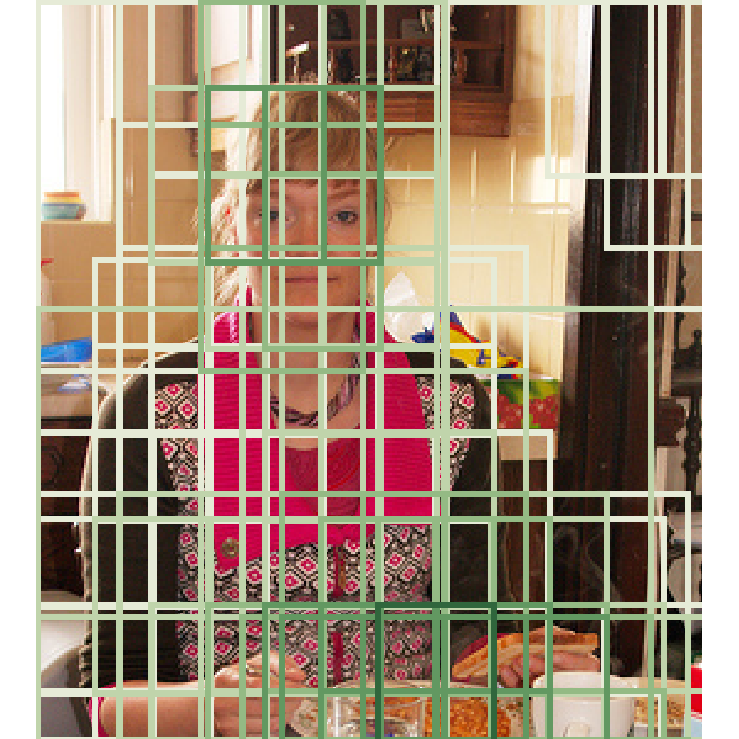
\includegraphics[width=0.47\textwidth]{figures/nms_before} &
        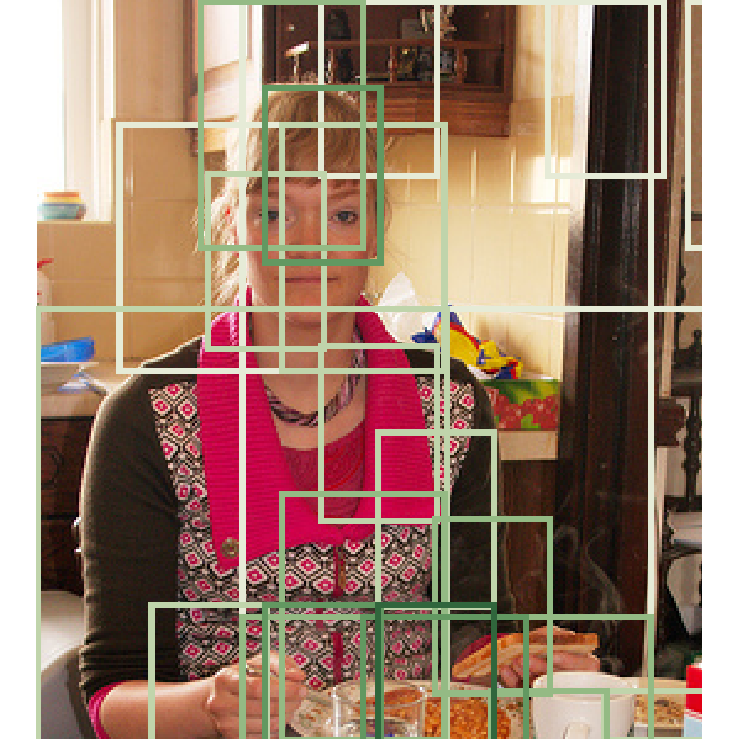
\includegraphics[width=0.47\textwidth]{figures/nms_after}
    \end{tabular}
	\caption{The effect of \acrfull{nms}.}
    \label{fig:nms}
\end{figure}
Depending on the number of scales, we generate hundreds or even thousands of boxes per image. We want to eliminate boxes that are overlapping with another box, which has a higher density. Firstly we drop the worst boxes $\{b_i: \rho_i < \rho_{min}\}$ with a low set threshold. While this is not necessary, it improves time performance and does not affect testing performance.\\
To the remaining boxes we apply \gls{nms}, as described by \citet{felzenszwalb_discriminatively_2008}. In the \gls{nms} we first sort all boxes by their scores $\rho_i$ in descending order, which in our case are the probability densities. We mark the strongest box as picked. Then we calculate the overlap in area between the new picked box and all remaining boxes. All boxes of which the area overlaps the picked box with 50\% or more are dropped. We pick the next strongest score of the remaining set and continue this process until all boxes are either dropped or picked. The strongest not-overlapping boxes remain picked and are returned. \figreft{fig:nms} shows the condensing effect of \gls{nms}.\\For minimal computational cost of this step we use the improved implementation from \citet{malisiewicz_ensemble_2011}.
